\documentclass[Eubank_pk_ethnic_sorting.tex]{subfiles}


\begin{document}

Having established that the determinants of school choice vary dramatically between caste-homogeneous and caste-heterogeneous villages in Section~\ref{pk_sorting}, this section now turns to an analysis of how differences in sorting impact the test-score gap between government and private schools. If private schools outperform government schools primarily due to differences in the quality of instruction, then the government-private test-score gap should be relatively stable across villages with different caste compositions. If, however, private schools appear to outperform government schools primarily due to differences in the composition of their students, then villages that are subject to different sorting processes should also see differences in the government-private test-score gap. Specifically, the degree to which private schools scores exceed those in government schools should decline as one moves from caste-homogeneous villages (where students sort on academic potential) to caste-heterogeneous villages (where sorting is driven by considerations of caste politics).

\subsection{Measuring Learning}\label{value_added_models}

To measure learning, this analysis employs a lagged-value-added model. Lagged-value-added models have increasingly become the norm in the education research \citep{Gordon:2006wt,McCaffrey:2003vk,Hanushek:2003hz} due to their potential to take into account not only observational differences between students, but also the potential to control for some unobserved differences, and the fact that learning is not entirely persistent (things learned in the past are often forgotten).

The lagged-value-added model incorporates the assumption that current knowledge is an additive function of all current and past inputs and an i.i.d. stochastic error term, and can be expressed as:

\begin{eqnarray}
	Y_{i,t}=X_{i,t}\alpha+Y_{i,t-1}\beta + \epsilon_{i,t}\label{primary}
\end{eqnarray}

where $Y_{i,t}$ is child $i$'s test scores at time $t$ and $X_{t,i}$ is a vector of child, school, and village controls at time $t$ (a full discussion of the lagged-value-added model, specifications employed, and identifying assumptions can be found in Appendix~\ref{appendix_valueadded}).

Note that while the inclusion of a lagged dependent variable effectively controls for unobserved heterogeneity that affect differences in test score \emph{levels}, it cannot control for unobserved heterogeneity that affects learning \emph{rates}. It is for this reason that while superior to other available methods, value-added analyses can not fully overcome selection issues.\footnote{Some analysis have turned to second-differencing the data and focusing on students who change schools \citep{Andrabi:2011hl}, but these analyses have their own limitations, among them limited sample sizes (given that changes between types of school are relatively infrequent in most surveys) and the assumption that school changes are not the result of some unobserved shock (i.e. that school switches are not accompanied by contemporaneous with other changes -- a potentially problematic assumption given the relative infrequency with which students change schools).} In the lagged-value-added model, coefficients on independent variables are interpreted as the contribution of each variable to learning.

\subsection{Convergence in Government-Private Test Scores}\label{}


Table~\ref{kids} presents lagged-valued-added estimates of learning as a function of various demographic controls and village fractionalization. It shows that the effect of caste fractionalization on the government-private test-score gap (row 2) is negative and significant for English and negative (albeit insignificant) for math and Urdu. Further, as shown in columns (2), (5), and (8) of Table~\ref{kids}, the inclusion of various demographic controls such as a child wealth index and dummies for parental education along with the village fixed effects has no significant effect on the results.


\begin{sidewaystable}[htbp]\centering
\def\sym#1{\ifmmode^{#1}\else\(^{#1}\)\fi}
\caption{Child Test Scores\label{kids}}
\begin{tabular}{l*{9}{c}}
\toprule
                &\multicolumn{3}{c}{English}           &\multicolumn{3}{c}{Urdu}              &\multicolumn{3}{c}{Math}              \\\cmidrule(lr){2-4}\cmidrule(lr){5-7}\cmidrule(lr){8-10}
                &\multicolumn{1}{c}{(1)}&\multicolumn{1}{c}{(2)}&\multicolumn{1}{c}{(3)}&\multicolumn{1}{c}{(4)}&\multicolumn{1}{c}{(5)}&\multicolumn{1}{c}{(6)}&\multicolumn{1}{c}{(7)}&\multicolumn{1}{c}{(8)}&\multicolumn{1}{c}{(9)}\\
                &\multicolumn{1}{c}{}&\multicolumn{1}{c}{}&\multicolumn{1}{c}{}&\multicolumn{1}{c}{}&\multicolumn{1}{c}{}&\multicolumn{1}{c}{}&\multicolumn{1}{c}{}&\multicolumn{1}{c}{}&\multicolumn{1}{c}{}\\
\midrule
Private School  &     0.63***&     0.60***&     0.59***&     0.27***&     0.26***&     0.20***&     0.19*  &     0.19*  &     0.12   \\
                &   (8.35)   &   (7.28)   &   (7.31)   &   (4.16)   &   (4.01)   &   (2.93)   &   (1.67)   &   (1.88)   &   (1.25)   \\
Fractionalization * Private&    -0.43***&    -0.41***&    -0.42***&    -0.17*  &    -0.17*  &   -0.094   &   -0.082   &    -0.12   &   -0.052   \\
                &  (-3.77)   &  (-3.46)   &  (-3.68)   &  (-1.71)   &  (-1.74)   &  (-0.98)   &  (-0.53)   &  (-0.83)   &  (-0.39)   \\
Lagged English Scores&     0.37***&     0.36***&     0.39***&     0.15***&     0.14***&     0.14***&     0.16***&     0.15***&     0.16***\\
                &  (21.16)   &  (20.03)   &  (20.61)   &  (13.05)   &  (11.37)   &  (11.69)   &  (10.78)   &  (10.06)   &   (9.86)   \\
Lagged Math Scores&    0.069***&    0.072***&    0.071***&     0.12***&     0.12***&     0.12***&     0.37***&     0.38***&     0.40***\\
                &   (8.55)   &   (8.91)   &   (8.49)   &  (14.10)   &  (13.51)   &  (13.96)   &  (29.56)   &  (27.37)   &  (28.76)   \\
Lagged Urdu Scores&     0.15***&     0.15***&     0.15***&     0.38***&     0.38***&     0.40***&     0.23***&     0.22***&     0.22***\\
                &  (14.04)   &  (13.28)   &  (12.71)   &  (34.36)   &  (32.65)   &  (31.74)   &  (17.67)   &  (17.01)   &  (16.84)   \\
Child's Wealth Index&            &    0.017***&    0.015***&            &   0.0073** &   0.0068** &            &    0.014***&    0.016***\\
                &            &   (5.19)   &   (4.29)   &            &   (2.46)   &   (2.28)   &            &   (3.52)   &   (3.73)   \\
Educated Parent &            &    0.058***&    0.053***&            &    0.052***&    0.049***&            &    0.046***&    0.043***\\
                &            &   (4.75)   &   (4.07)   &            &   (4.77)   &   (4.40)   &            &   (3.35)   &   (3.08)   \\
Biraderi Fractionalization&            &            &     0.21** &            &            &    0.095   &            &            &     0.14   \\
                &            &            &   (2.56)   &            &            &   (1.40)   &            &            &   (1.38)   \\
Village: Pct Adults Literate&            &            &  0.00017   &            &            & -0.00054   &            &            &  0.00036   \\
                &            &            &   (0.18)   &            &            &  (-0.62)   &            &            &   (0.27)   \\
Log Village Size&            &            &    0.019   &            &            &    0.014   &            &            &   0.0088   \\
                &            &            &   (1.47)   &            &            &   (1.01)   &            &            &   (0.50)   \\
Village Land Gini&            &            &    0.053   &            &            &    0.061   &            &            &    -0.25*  \\
                &            &            &   (0.47)   &            &            &   (0.63)   &            &            &  (-1.88)   \\
Constant        &     0.25   &     0.40*  &     0.57** &     0.56** &     0.69***&     0.78***&     0.12   &     0.31   &     0.60*  \\
                &   (0.99)   &   (1.78)   &   (2.28)   &   (2.58)   &   (2.78)   &   (2.80)   &   (0.37)   &   (0.99)   &   (1.74)   \\
Village Fixed Effects&      Yes   &      Yes   &       No   &      Yes   &      Yes   &       No   &      Yes   &      Yes   &       No   \\
District Fixed Effects&       No   &       No   &      Yes   &       No   &       No   &      Yes   &       No   &       No   &      Yes   \\
\midrule
Observations    &    37147   &    26141   &    26141   &    37147   &    26141   &    26141   &    37147   &    26141   &    26141   \\
\bottomrule
\multicolumn{10}{l}{\footnotesize Controls for age, age squared, gender, and class omitted from table. Standard errors clustered at village level.}\\
\multicolumn{10}{l}{\footnotesize * p<0.10, ** p<0.05, *** p<0.01}\\
\end{tabular}
\end{sidewaystable}


To aid in interpretation, Figure~\ref{kidscombined} plots the government-private performance differential as a function of caste fractionalization (these plots correspond to columns (2), (5), and (8) respectively). In all three cases, the rise in fractionalization is associated with a near 50\% decline in the private school premium, although this is by far most striking in the case of English.

The differential impact of village fragmentation on English and other subjects is not surprising. English is generally considered the path to upward mobility in Pakistan, and is often the focus of private schools in Punjab. For example, while only 6\% of government schools use English as one of their languages of instruction, this is the case in 28\% of private schools \citep[p. 49]{Andrabi:2007we}. Indeed, a consistent pattern in the data is that -- possibly as a result of this specialization -- the English test-score gap is consistently the largest among the three subjects tested. 

\begin{figure}[h]
	\caption{Private School Test Score Premium with Lagged Scores}\label{kidscombined}
	\centering
	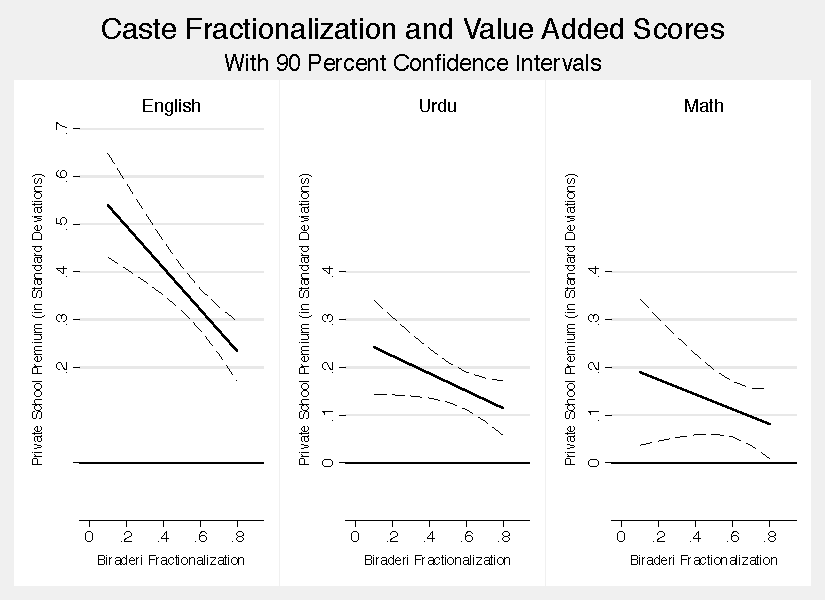
\includegraphics[scale=0.8]{../results/kids_combined.pdf}
\end{figure}


\subsection{Decomposition of Convergence}\label{village_level_outcomes}

Further evidence that the convergence in government-private test scores is driven differences in student sorting -- not differences in actual learning outcomes -- comes from the fact that while the government-private test-gap decreases, overall learning remains relatively unchanged across villages. As shown in Table~\ref{kidsnointeract} -- which examines the relationship between overall test scores and village heterogeneity -- test scores do not vary with caste composition. English scores are slightly higher in more fractionalized villages in Column 1, but the magnitude of this difference is relatively small, and once more demographic controls are added in Column 2 this effect disappears. No relationship exists for other subjects. Government scores increase and private scores decline with fractionalization, in other words, but those changes are almost perfectly offsetting. 


\begin{sidewaystable}[htbp]\centering
\def\sym#1{\ifmmode^{#1}\else\(^{#1}\)\fi}
\caption{Child Test Scores and Fractionalization \label{kidsnointeract}}
\begin{tabular}{l*{6}{c}}
\toprule
                &\multicolumn{2}{c}{English}&\multicolumn{2}{c}{Urdu} &\multicolumn{2}{c}{Math} \\\cmidrule(lr){2-3}\cmidrule(lr){4-5}\cmidrule(lr){6-7}
                &\multicolumn{1}{c}{(1)}&\multicolumn{1}{c}{(2)}&\multicolumn{1}{c}{(3)}&\multicolumn{1}{c}{(4)}&\multicolumn{1}{c}{(5)}&\multicolumn{1}{c}{(6)}\\
                &\multicolumn{1}{c}{}&\multicolumn{1}{c}{}&\multicolumn{1}{c}{}&\multicolumn{1}{c}{}&\multicolumn{1}{c}{}&\multicolumn{1}{c}{}\\
\midrule
Private School  &     0.31***&     0.29***&     0.14***&     0.14***&     0.11***&    0.087** \\
                &  (10.98)   &  (10.42)   &   (5.74)   &   (5.65)   &   (3.17)   &   (2.58)   \\
Biraderi Fractionalization&     0.13*  &    0.096   &    0.085   &    0.069   &     0.13   &     0.13   \\
                &   (1.70)   &   (1.33)   &   (1.26)   &   (1.08)   &   (1.34)   &   (1.46)   \\
Lagged English Scores&     0.40***&     0.39***&     0.16***&     0.14***&     0.17***&     0.16***\\
                &  (22.32)   &  (21.10)   &  (13.39)   &  (11.90)   &  (10.27)   &   (9.92)   \\
Lagged Math Scores&    0.067***&    0.070***&     0.12***&     0.12***&     0.39***&     0.40***\\
                &   (8.18)   &   (8.37)   &  (14.51)   &  (14.00)   &  (30.92)   &  (28.87)   \\
Lagged Urdu Scores&     0.15***&     0.15***&     0.39***&     0.40***&     0.23***&     0.22***\\
                &  (13.26)   &  (12.80)   &  (34.01)   &  (31.76)   &  (17.96)   &  (16.86)   \\
Village: Pct Adults Literate&  0.00067   &  0.00022   & -0.00018   & -0.00053   &  0.00043   &  0.00036   \\
                &   (0.68)   &   (0.23)   &  (-0.21)   &  (-0.61)   &   (0.31)   &   (0.27)   \\
Log Number of Households&    0.017   &    0.019   &    0.011   &    0.014   &   0.0070   &   0.0087   \\
                &   (1.33)   &   (1.39)   &   (0.73)   &   (1.01)   &   (0.35)   &   (0.50)   \\
Village Land Gini&   0.0097   &    0.045   &    0.013   &    0.059   &    -0.28** &    -0.25*  \\
                &   (0.08)   &   (0.39)   &   (0.13)   &   (0.61)   &  (-2.22)   &  (-1.90)   \\
Child's Wealth Index&            &    0.015***&            &   0.0068** &            &    0.016***\\
                &            &   (4.22)   &            &   (2.27)   &            &   (3.73)   \\
Educated Parent &            &    0.053***&            &    0.049***&            &    0.043***\\
                &            &   (4.13)   &            &   (4.42)   &            &   (3.08)   \\
Constant        &     0.44   &     0.22   &     0.67***&     0.62   &     0.32   &     0.91   \\
                &   (1.57)   &        .   &   (2.65)   &        .   &   (0.87)   &   (0.00)   \\
District Fixed Effects&      Yes   &      Yes   &      Yes   &      Yes   &      Yes   &      Yes   \\
\midrule
Observations    &    37147   &    26141   &    37147   &    26141   &    37147   &    26141   \\
\bottomrule
\multicolumn{7}{l}{\footnotesize \textit{t} statistics in parentheses}\\
\multicolumn{7}{l}{\footnotesize * p<0.10, ** p<0.05, *** p<0.01}\\
\end{tabular}
\end{sidewaystable}



\subsection{Caste and Residual Academic Potential}\label{residual_potential}

For it to be the case that sorting by caste reduces the degree to which private schools enroll disproportionately academically-inclined students, residual academic potential -- potential that cannot be explained by things like parental education and wealth -- must be equally distributed across different castes (or be distributed slightly in favor of lower status \emph{biraderis}). If not, and even the least talented ``high status'' students were more talented than the most talented ``low status'' students, then the concentration of ``high status'' students in private schools would result in \emph{divergence}, rather than \emph{convergence}, of test scores. As shown in Table~\ref{castesarentdumb}, however, there is no evidence that those from higher social status \emph{biraderis} have higher residual talent than those from low status \emph{biraderis}. As evident from the top row of coefficients, after controlling for other observational factors, student caste does not appear to have any consistent effect on test scores.

\begin{sidewaystable}[htbp]\centering
\def\sym#1{\ifmmode^{#1}\else\(^{#1}\)\fi}
\caption{Child Social Status and Residual Talent\label{castesarentdumb}}
\begin{tabular}{l*{9}{c}}
\toprule
                &\multicolumn{3}{c}{English}           &\multicolumn{3}{c}{Urdu}              &\multicolumn{3}{c}{Math}              \\\cmidrule(lr){2-4}\cmidrule(lr){5-7}\cmidrule(lr){8-10}
                &\multicolumn{1}{c}{(1)}&\multicolumn{1}{c}{(2)}&\multicolumn{1}{c}{(3)}&\multicolumn{1}{c}{(4)}&\multicolumn{1}{c}{(5)}&\multicolumn{1}{c}{(6)}&\multicolumn{1}{c}{(7)}&\multicolumn{1}{c}{(8)}&\multicolumn{1}{c}{(9)}\\
                &\multicolumn{1}{c}{}&\multicolumn{1}{c}{}&\multicolumn{1}{c}{}&\multicolumn{1}{c}{}&\multicolumn{1}{c}{}&\multicolumn{1}{c}{}&\multicolumn{1}{c}{}&\multicolumn{1}{c}{}&\multicolumn{1}{c}{}\\
\midrule
High Status Biraderi&   -0.035   &   -0.062   &    -0.11** &   -0.044   &    -0.11   &   -0.081   &   0.0056   &   -0.019   &    0.034   \\
                &  (-0.79)   &  (-0.93)   &  (-2.41)   &  (-0.75)   &  (-1.55)   &  (-1.61)   &   (0.09)   &  (-0.22)   &   (0.50)   \\
Private School  &     0.30** &     0.20   &     0.18   &     0.22*  &     0.18   &    0.026   &    -0.10   &    -0.13   &    -0.24   \\
                &   (2.53)   &   (1.50)   &   (1.46)   &   (1.92)   &   (1.37)   &   (0.21)   &  (-0.96)   &  (-0.96)   &  (-1.55)   \\
Fractionalization * Private&   0.0010   &     0.12   &    0.100   &   -0.097   &   -0.057   &     0.11   &     0.35** &     0.42*  &     0.47** \\
                &   (0.01)   &   (0.60)   &   (0.54)   &  (-0.60)   &  (-0.29)   &   (0.63)   &   (2.02)   &   (1.97)   &   (2.13)   \\
Lagged English Scores&     0.32***&     0.31***&     0.40***&     0.15***&     0.15***&     0.15***&     0.17***&     0.17***&     0.16***\\
                &   (7.79)   &   (6.95)   &  (10.37)   &   (4.80)   &   (4.19)   &   (5.12)   &   (3.81)   &   (3.74)   &   (3.93)   \\
Lagged Math Scores&    0.066** &    0.061*  &    0.050   &     0.12***&    0.094** &     0.10** &     0.31***&     0.29***&     0.38***\\
                &   (2.21)   &   (1.68)   &   (1.51)   &   (3.04)   &   (2.23)   &   (2.57)   &   (6.38)   &   (5.93)   &   (8.33)   \\
Lagged Urdu Scores&     0.17***&     0.18***&     0.16***&     0.34***&     0.35***&     0.40***&     0.25***&     0.25***&     0.25***\\
                &   (4.72)   &   (4.11)   &   (4.04)   &   (8.85)   &   (7.57)   &   (8.74)   &   (5.51)   &   (4.96)   &   (4.94)   \\
Child's Wealth Index&            &  -0.0055   &  -0.0080   &            &   0.0060   &   0.0046   &            &  -0.0094   &  -0.0062   \\
                &            &  (-0.43)   &  (-0.69)   &            &   (0.57)   &   (0.52)   &            &  (-0.57)   &  (-0.44)   \\
Educated Parent &            &     0.12***&     0.13***&            &     0.14***&     0.14***&            &     0.15***&     0.17***\\
                &            &   (2.95)   &   (3.52)   &            &   (3.25)   &   (4.01)   &            &   (2.85)   &   (3.68)   \\
Biraderi Fractionalization&            &            &  -0.0096   &            &            &   -0.076   &            &            &   -0.024   \\
                &            &            &  (-0.09)   &            &            &  (-0.70)   &            &            &  (-0.16)   \\
Village: Pct Adults Literate&            &            &0.00000016   &            &            &  -0.0030** &            &            &  -0.0022   \\
                &            &            &   (0.00)   &            &            &  (-2.03)   &            &            &  (-0.84)   \\
Log Village Size&            &            &    0.011   &            &            &    0.016   &            &            &    0.026   \\
                &            &            &   (0.33)   &            &            &   (0.52)   &            &            &   (0.44)   \\
Village Land Gini&            &            &   -0.031   &            &            &    0.054   &            &            &    -0.11   \\
                &            &            &  (-0.17)   &            &            &   (0.28)   &            &            &  (-0.37)   \\
Constant        &    -0.62   &     0.20   &     1.00*  &    -0.15   &     2.16***&     2.28***&    -0.71   &     2.98***&     2.59***\\
                &  (-1.25)   &   (0.29)   &   (1.71)   &  (-0.26)   &   (3.07)   &   (3.46)   &  (-1.07)   &   (3.44)   &   (2.90)   \\
Village Fixed Effects&      Yes   &      Yes   &       No   &      Yes   &      Yes   &       No   &      Yes   &      Yes   &       No   \\
District Fixed Effects&       No   &       No   &      Yes   &       No   &       No   &      Yes   &       No   &       No   &      Yes   \\
\midrule
Observations    &     1859   &     1381   &     1381   &     1859   &     1381   &     1381   &     1859   &     1381   &     1381   \\
\bottomrule
\multicolumn{10}{l}{\footnotesize Controls for age, age squared, gender, and class omitted from table. Standard errors clustered at village level.}\\
\multicolumn{10}{l}{\footnotesize * p<0.10, ** p<0.05, *** p<0.01}\\
\end{tabular}
\end{sidewaystable}



\end{document}
